\documentclass{beamer}

% \usetheme{Pittsburgh}
 \setbeamertemplate{enumerate items}[circle]
%  \usetheme{Boadilla}
\usepackage[ngerman,english]{babel}			
\usepackage[utf8]{inputenc}				

\usepackage{color}
\usepackage{booktabs}
\usepackage{animate}
\usepackage{hyperref}
\usepackage{dirtytalk} % quotes
\usepackage{amsmath}
\usepackage{bm}

% \usepackage{natbib}
% \usepackage{apalike}
% \bibliography{refs}

\usepackage[style=apa]{biblatex}
\addbibresource{refs.bib}

% Define command to print full bibliography in footnote
\newcommand{\fcite}[1]{\footnote{\fullcite{#1}}}

\hypersetup{colorlinks,urlcolor=blue, linkcolor=blue}

\setbeamertemplate{footline}[frame number]
\setbeamertemplate{section in toc}[sections numbered]
\setcounter{tocdepth}{2}
% \setbeamertemplate{subsection in toc}[subsections numbered]

% LOGO TOP RIGHT
% \usepackage{tikz}
% \titlegraphic { 
% \begin{tikzpicture}[overlay,remember picture]
% \node[left=0.2cm] at (current page.30){
%     
\includegraphics[width=3cm]{figures/mpidr_logo_colour_de_1.png}
% };
% \end{tikzpicture}
% }

% LOGO BOTTOM RIGHT
\titlegraphic{

\includegraphics[width=5cm]{figures/mpidr_logo_colour_de_1.png}
\hfill

\includegraphics[width=3cm]{figures/edsd-logo.png}
}

% \makeatletter
% \setbeamertemplate{navigation symbols}{}

% make blocks no transparent
\setbeamercolor{block body alerted}{bg=alerted text.fg!10}
\setbeamercolor{block title alerted}{bg=alerted text.fg!20}
\setbeamercolor{block body}{bg=structure!10}
\setbeamercolor{block title}{bg=structure!20}
\setbeamercolor{block body example}{bg=green!10}
\setbeamercolor{block title example}{bg=green!20}



%%	title page information

\title[Kinship]{Kinship Structures (3)}
\subtitle{Extensions of the kinship model}

\author{Diego Alburez Guti\'errez$^{\dagger}$}

\institute{$^{\dagger}$Kinship Inequalities Research Group, \\ Max Planck Institute for Demographic Research }

\date{European Doctoral School of Demography 2025-26 \\ 4 Mar 2026}

%%	Begin of the document:
%%	======================

\begin{document}

 \begin{frame}[t,plain]
 \titlepage
 \end{frame}

 
\begin{frame}{Agenda}
\tableofcontents
\end{frame}

\begin{frame}{Recap}
    \begin{enumerate}
        \item What is the general form of the (time-invariant) kinship models?
        \item What are the different `model specifications' that we discussed yesterday?
    \end{enumerate}
\end{frame}

\begin{frame}{Typology of kinship models}

\begin{table}[]
\begin{tabular}{@{}lllll@{}}
\toprule
No & time      & sex    & state    & reference \\ \midrule
1 & invariant & female & age & \\ 
2 & variant   & female & age &  \\
3 & invariant & two   & age &  \\
4 & invariant   & female   &  multiple &  \\ 
5 & variant   & two   &  multiple & \\ \bottomrule
\end{tabular}
\end{table}

\end{frame}

\section{Time-variance}
\begin{frame}
    \begin{centering}
    \begin{beamercolorbox}[sep=12pt,center]{part title}
    \usebeamerfont{section title}\insertsection\par
    \end{beamercolorbox}
    \end{centering}
\end{frame}

\begin{frame}{Typology of kinship models}

\begin{table}[]
\begin{tabular}{@{}lllll@{}}
\toprule
No & time      & sex    & state    & reference \\ \midrule
1 & invariant & female & age & \\ 
\textbf{2} & \textbf{variant}   & \textbf{female} & \textbf{age} & \fcite{caswell_formal_2021} \\
3 & invariant & two   & age & \\
4 & invariant   & female   &  multiple & \\ 
5 & variant   & two   &  multiple & \\ \bottomrule
\end{tabular}
\end{table}

\end{frame}

\begin{frame}{Time-variant kinship models}
    \begin{enumerate}
        \item Demographic rates change over time
        \item Past demographic change $\rightarrow$ contemporary kinship structures
        \item E.g., mortality crises, baby booms
        \item Estimates by age, period, and cohort  
    \end{enumerate}
\end{frame}

\begin{frame}{Recap: Time-invariant, one-sex model}
    The models are of the general form:

\begin{equation*}
    	\underbrace{{\bf k}(x+1)}_{\substack{\text{age structure of kin}\\ \text{at Focal's age $x+1$}}} = 	
    \underbrace{{\bf U \, k}(x)}_{\substack{\text{ageing and survival}\\ \text{of existing kin}}}
    + 	\underbrace{	\left\{ \begin{array}{l}
    \bm 0 \\
    {\bf F \, k}^*(x)
    \end{array}
    \right.}_{\substack{\text{new kin members}\\ \text{added to the population}}}.
\end{equation*}

where:
\vspace{.2cm}
\begin{itemize}
    \item ${\bf U}$ a matrix with survival probabilities in the subdiagonal
    \item ${\bf F}$ a matrix with fertility rates in the first row
\end{itemize}

\end{frame}

\begin{frame}{Time-variant, one-sex model}
    The models are of the general form:

\begin{equation*}
    	\underbrace{{\bf k}(x+1,t+1)}_{\substack{\text{age structure of kin}\\ \text{at Focal's age $x+1$} \\ \text{and time $t+1$} }} = 	
    \underbrace{{\bf U_t \, k}(x,t)}_{\substack{\text{ageing and survival}\\ \text{of existing kin}}}
    + 	\underbrace{	\left\{ \begin{array}{l}
    \bm 0 \\
    {\bf F_t \, k}^*(x,t)
    \end{array}
    \right.}_{\substack{\text{new kin members}\\ \text{added to the population}}}.
\end{equation*}

where:
\vspace{.2cm}
\begin{itemize}
    \item ${\bf U_t}$ a matrix with time-variant survival probabilities in the subdiagonal
    \item ${\bf F_t}$ a matrix with time-variant fertility rates in the first row
\end{itemize}

\end{frame}

\begin{frame}{Boundary conditions}
              \begin{figure}[!h]
      \centering
      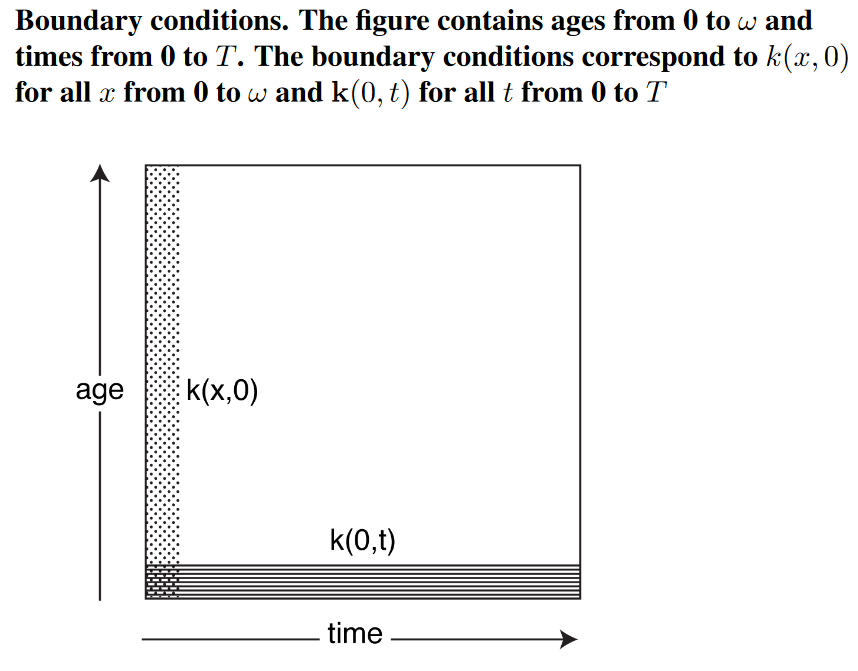
\includegraphics[width =.9\textwidth]{figures/boundary.PNG}
     \end{figure} 
\end{frame}

\begin{frame}{Boundary conditions}

\begin{itemize}
    \item specify the complete age vector at time $t = 0$
\end{itemize}

\begin{equation*}
    {\bf k}(x,0) \qquad x = 0, ..., \omega.
\end{equation*}

\begin{itemize}
    \item Specify the initial vector at each time
\end{itemize}

\begin{equation*}
    {\bf k}(0,t) \qquad t = 0, ..., \omega.
\end{equation*}

\end{frame}

\begin{frame}{Daughters}

Daughters ($\bf a$) are the result of the reproduction of Focal:

    \begin{equation}
    	\underbrace{{\bf a}(x+1,t+1)}_{\substack{\text{age structure of daughters}\\ \text{at Focal's age $x+1$}}} = 	
    \underbrace{{\bf U_t \, a}(x,t)}_{\substack{\text{ageing and survival}\\ \text{of existing daughters}}}
    + 	\underbrace{	{\bf F_t \, e}_x.}_{\substack{\text{new daughters}\\ \text{(subsidy)}}}
\end{equation}

\begin{equation*}
    a(0) = {\bf 0}.
\end{equation*}

where:
\begin{itemize}
    \item ${\bf U_t}$ is a matrix with time-variant survival probabilities in the subdiagonal
    \item ${\bf F_t}$ is a matrix with time-variant fertility rates in the first row
    \item ${\bf F_t \, e}_x$ is the subsidy vector
    \item $e_x$ is the unit vector for age $x$
    \item $a(0)$ is the distribution of daughters at Focal's birth
\end{itemize}

\end{frame}

\begin{frame}{Mothers}

 The population of mothers ($\bf d$) of Focal consists of at most a single
individual:

    \begin{equation}
    	\underbrace{{\bf d}(x+1,t+1)}_{\substack{\text{age structure of mothers}\\ \text{at Focal's age $x+1$}}} = 	
    \underbrace{{\bf U_t \, d}(x,t)}_{\substack{\text{ageing and survival}\\ \text{of existing mothers}}}
    + 	\underbrace{	{\bf 0}.}_{\substack{\text{new mothers}\\ \text{(subsidy)}}}
\end{equation}

\begin{equation*}
    d(0) = {\bf \pi}(t).
\end{equation*}

where:
\begin{itemize}
    \item $b(0)$ is the distribution of mothers at Focal's birth
    \item ${\bf \pi}(t)$ is the distribution of ages of mothers in the population
\end{itemize}

\end{frame}

\begin{frame}{Age, period, and cohort in kinship models}
          \begin{figure}[!h]
      \centering
      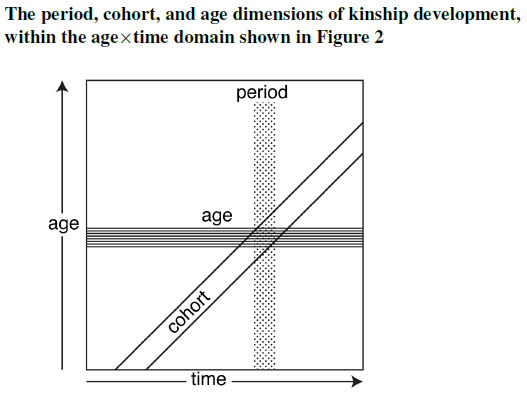
\includegraphics[width =.9\textwidth]{figures/cohort.png}
     \end{figure} 
\end{frame}

\begin{frame}{Period results for numbers of daughters and granddaughters in Sweden}
          \begin{figure}[!h]
      \centering
      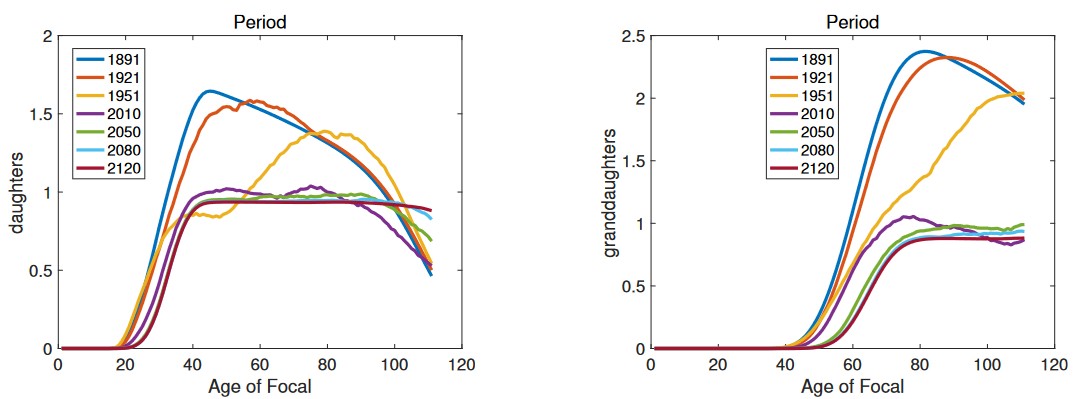
\includegraphics[width =1\textwidth]{figures/pe.PNG}
     \end{figure} 
\end{frame}

\begin{frame}{Cohort results for numbers of daughters and granddaughters in Sweden}
          \begin{figure}[!h]
      \centering
      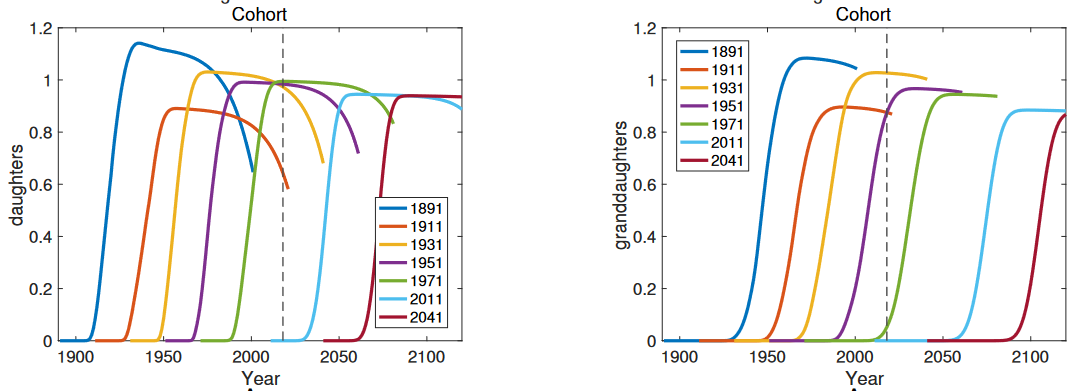
\includegraphics[width =1\textwidth]{figures/co.PNG}
     \end{figure} 
\end{frame}

\begin{frame}{Age results for numbers of daughters and granddaughters in Sweden}
          \begin{figure}[!h]
      \centering
      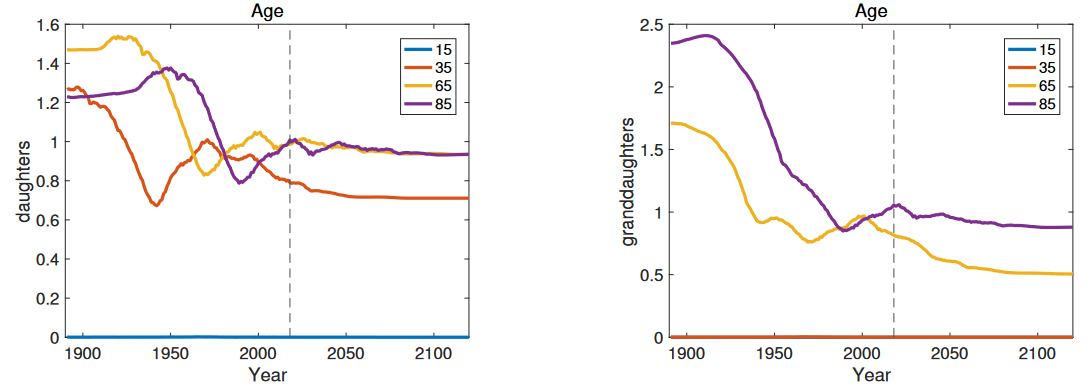
\includegraphics[width =1\textwidth]{figures/age.PNG}
     \end{figure} 
\end{frame}

\begin{frame}{Discuss}
    \begin{enumerate}
        \item What is the difference between the expected number of daughters calculated using (i) a time-invariant model, and (ii) the period dimension of the time-variant model?
        \item What is the difference between the period and cohort results of the time-variant model?
        \item How do the time-variant models deal with missing demographic data before a certain year (e.g., the UN only reports data starting in 1950)?
    \end{enumerate}
\end{frame}

\begin{frame}{}
    \centering
    \huge Break
\end{frame}

\section{Two-sex models}
\begin{frame}
    \begin{centering}
    \begin{beamercolorbox}[sep=12pt,center]{part title}
    \usebeamerfont{section title}\insertsection\par
    \end{beamercolorbox}
    \end{centering}
\end{frame}

\begin{frame}{Typology of kinship models}
\begin{table}[]
\begin{tabular}{@{}lllll@{}}
\toprule
No & time      & sex    & state    & reference \\ \midrule
1 & invariant & female & age & \\ 
2 & variant   & female & age & \\
\textbf{3} & \textbf{invariant} & \textbf{two}   & \textbf{age} & \fcite{caswell_formal_2022} \\
4 & invariant   & female   &  multiple & \\ 
5 & variant   & two   &  multiple & \\ \bottomrule
\end{tabular}
\end{table}
\end{frame}

\begin{frame}{Why do we need two-sex models?}
    \begin{enumerate}
        \item Differential survival and reproduction for women and men
        \item These differences are not stable: change over time
        \item More pronounced in some settings
        \item Estimate male and female kin for  male and female Focals
    \end{enumerate}
\end{frame}

\begin{frame}{Two-sex model (descendants)}
                 \begin{figure}[!h]
      \centering
      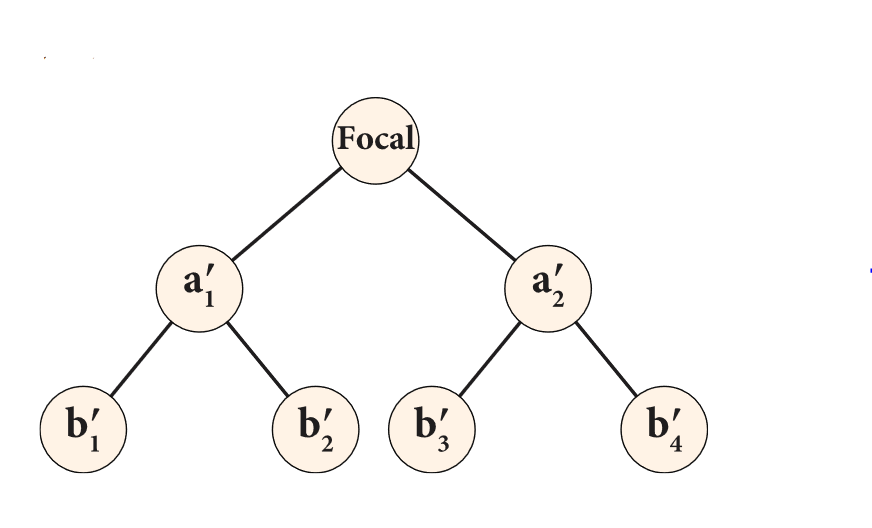
\includegraphics[width =.6\textwidth]{figures/two.PNG}
     \end{figure} 

\begin{equation*}
    {\bf \tilde{a}} = \begin{pmatrix}
        {\bf a'}_1 \\
        {\bf a'}_2
    \end{pmatrix}
\end{equation*}

     where
     \begin{itemize}
         \item ${\bf \tilde{a}}$ is a block-structured matrix of the expected number of living offspring
         \item $ {\bf a'}_1$ is the expected number of living sons
         \item $ {\bf a'}_2$ is the expected number of living daughters
     \end{itemize}
\end{frame}

\begin{frame}{Offspring (sons and daughters)}

Children ($\bf \tilde{a}$) are the result of the reproduction of Focal:

    \begin{equation}
    	\underbrace{{\bf \tilde{a}}(x+1)}_{\substack{\text{age structure of offspring}\\ \text{at Focal's age $x+1$}}} = 	
    \underbrace{{\bf \tilde{U} \, \tilde{a}}(x)}_{\substack{\text{ageing and survival}\\ \text{of existing offspring}}}
    + 	\underbrace{	{\bf \tilde{F} \, \tilde{\phi} }(x).}_{\substack{\text{new offspring}\\ \text{(subsidy)}}}
\end{equation}

\begin{equation*}
    \tilde{a}(0) = {\bf 0}.
\end{equation*}

where:
\begin{itemize}
    \item ${\bf \tilde{U}}$ is a block-structured matrix of survival probabilities
    \item ${\bf \tilde{F}}$ is a block-structured matrix of fertility rates
    \item ${\bf \tilde{F} \, \tilde{\phi} }(x)$ is the subsidy vector
    \item $\tilde{\phi}(x)$ is the state vector of a Focal of specified sex 
    \item $\tilde{a}(0)$ is the distribution of offspring at Focal's birth
\end{itemize}

\end{frame}

\begin{frame}{Blocks-structured input matrices}

For mortality: 

\begin{equation*}
    {\bf \tilde{U}} = \begin{pmatrix}
    {\bf U}_f & {\bf 0} \\
    {\bf 0} & {\bf U}_m
    \end{pmatrix}
\end{equation*}

\vspace{1cm}

For fertility:

\begin{equation*}
    {\bf \tilde{F}} = \begin{pmatrix}
    {\bf \bar{\alpha} F}_f & {\bf \bar{\alpha} F}_m \\
    {\bf \alpha F}_f & {\bf \bar{\alpha} F}_m
    \end{pmatrix}
\end{equation*}

    where
    \begin{itemize}
        \item ${\bf U}_f$ is a matrix with female survival probabilities in the subdiagonal
        \item ${\bf F}_f$ is a matrix with female fertility rates in the first row 
        \item $\alpha$ is the proportion males among offspring
        \item $\bar{\alpha}$ is $1-\alpha$
    \end{itemize}
\end{frame}

\begin{frame}{Parents}

The population of parents ($\bf \tilde{d}$) of Focal consists of at most a single
individual:

    \begin{equation}
    	\underbrace{{\bf \tilde{d}}(x+1)}_{\substack{\text{age structure of parents}\\ \text{at Focal's age $x+1$}}} = 	
    \underbrace{{\bf \tilde{U} \, \tilde{d}}(x)}_{\substack{\text{ageing and survival}\\ \text{of existing parents}}}
    + 	\underbrace{	{\bf 0}.}_{\substack{\text{new parents}\\ \text{(subsidy)}}}
\end{equation}

\begin{equation*}
    \tilde{d}(0) = {\bf \tilde{\pi}}.
\end{equation*}

where:
\begin{itemize}
    \item $\tilde{b}(0)$ is the distribution of parents at Focal's birth
    \item ${\bf \tilde{\pi}}$ is the distribution of ages of parents in the population
\end{itemize}
\end{frame}

\begin{frame}{Two-sex kin estimation}
             \begin{figure}[!h]
      \centering
      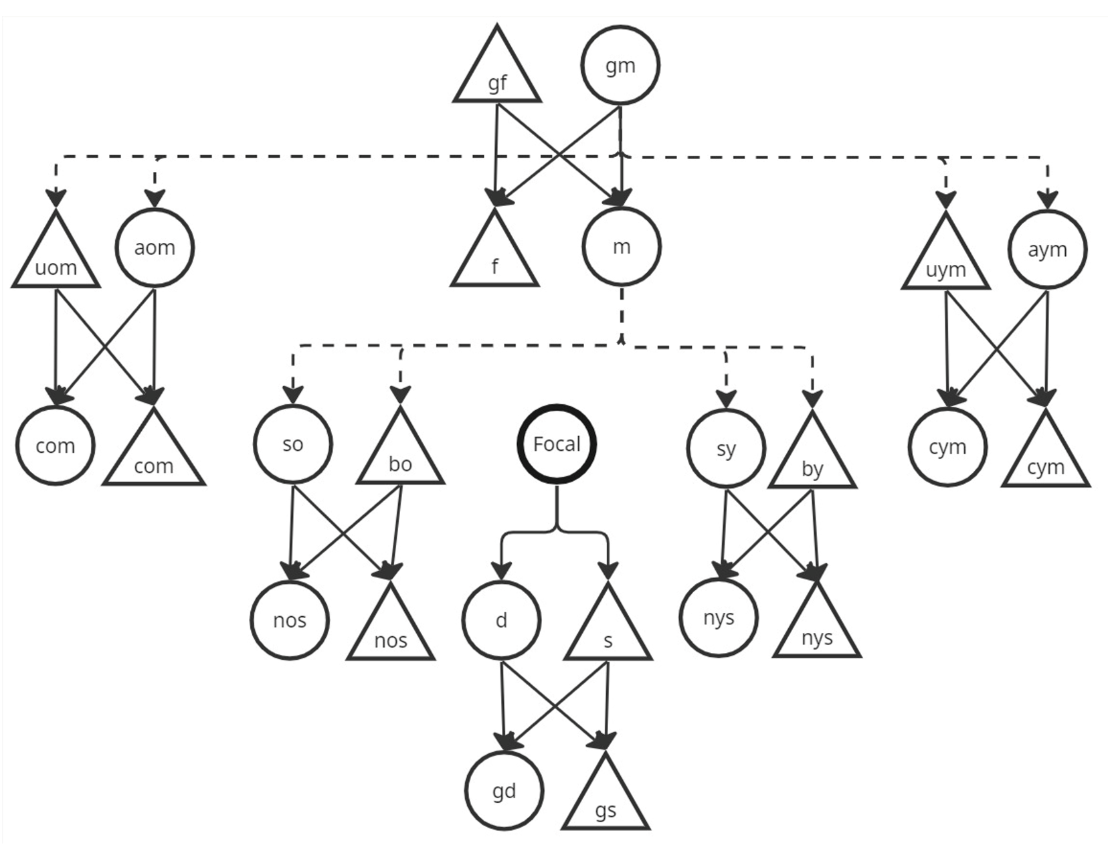
\includegraphics[width =1\textwidth]{figures/tree.PNG}
     \end{figure} 
\end{frame}

\begin{frame}{Data requirements}
             \begin{figure}[!h]
      \centering
      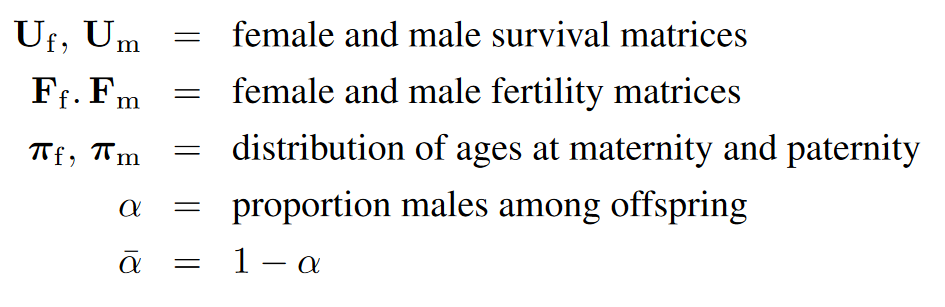
\includegraphics[width =.9\textwidth]{figures/input.PNG}
     \end{figure} 
\end{frame}


\begin{frame}{Male and female fertility}
     \begin{figure}[!h]
      \centering
      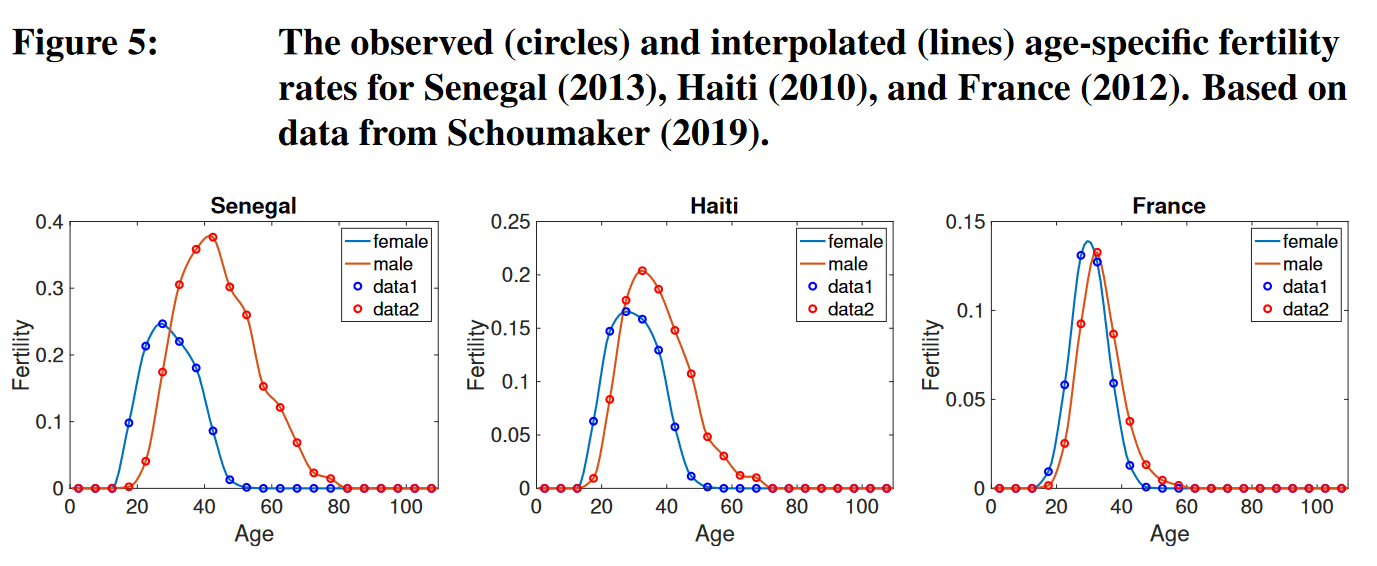
\includegraphics[width =1\textwidth]{figures/fert.PNG}
     \end{figure} 
\end{frame}

\begin{frame}{Approximations for two-sex kinship models}
    \begin{enumerate}
        \item Androgynous fertility
        \begin{itemize}
            \item Assume that ${\bf F}_m = {\bf F}_f$
        \end{itemize}
        \item GKP factors
        \begin{itemize}
            \item Run one-sex model and multiply resulting kinship structure by a `GKP factor'
            \item daughters $\times$ 2, granddaughters $\times$ 4, great-granddaughters $\times$ 8, mothers $\times$ 2, grandmothers $\times$ 4, great-grandmothers $\times$ 8, sisters $\times$ 2, nieces $\times$ 4, aunts $\times$ 4, and cousins $\times$ 8
        \end{itemize}
    \end{enumerate}
\end{frame}

\begin{frame}{Expected number of female and male kin in three countries}
     \begin{figure}[!h]
      \centering
      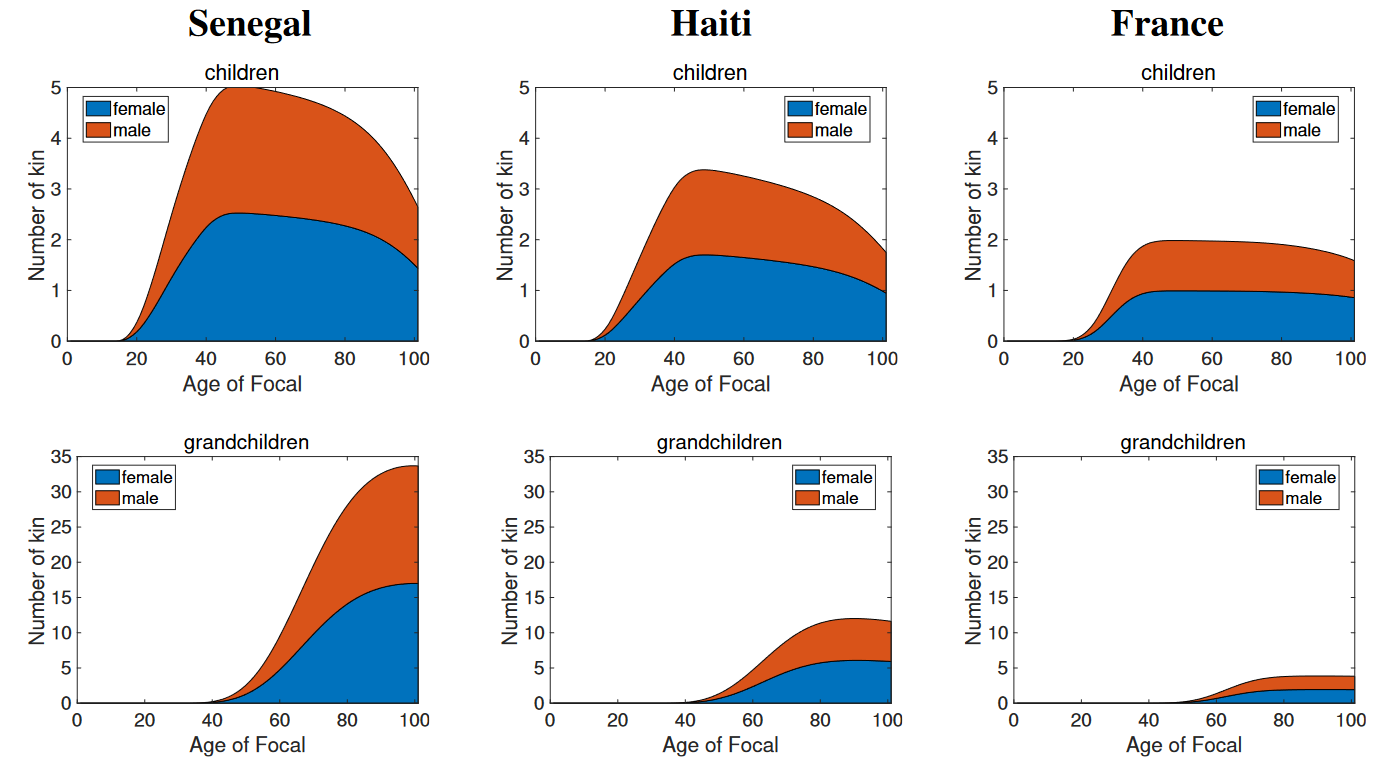
\includegraphics[width =.9\textwidth]{figures/two-ex.PNG}
     \end{figure} 
\end{frame}

\begin{frame}{Discuss}
    \begin{enumerate}
        \item Why do we need the `androgynous' and `GKP factor' approximations for two-sex kinship models?
        \item Which of the two do you think is better? Can you think of other possible `approximations'?
    \end{enumerate}
\end{frame}

\section{Other extensions}
\begin{frame}
    \begin{centering}
    \begin{beamercolorbox}[sep=12pt,center]{part title}
    \usebeamerfont{section title}\insertsection\par
    \end{beamercolorbox}
    \end{centering}
\end{frame}

\begin{frame}{Typology of kinship models}
\begin{table}[]
\begin{tabular}{@{}lllll@{}}
\toprule
No & time      & sex    & state    & reference \\ \midrule
1 & invariant & female & age & \\ 
2 & variant   & female & age & \\
3 & invariant & two   & age & \\
4 & invariant & female   &  multiple & \\
5 & \textbf{variant}   & two   &  \textbf{multiple} & \fcite{williams_demokin_2023} \\ \bottomrule
\end{tabular}
\end{table}
\end{frame}

\begin{frame}{Multistate kinship models}    
      \begin{figure}[!h]
      \centering
      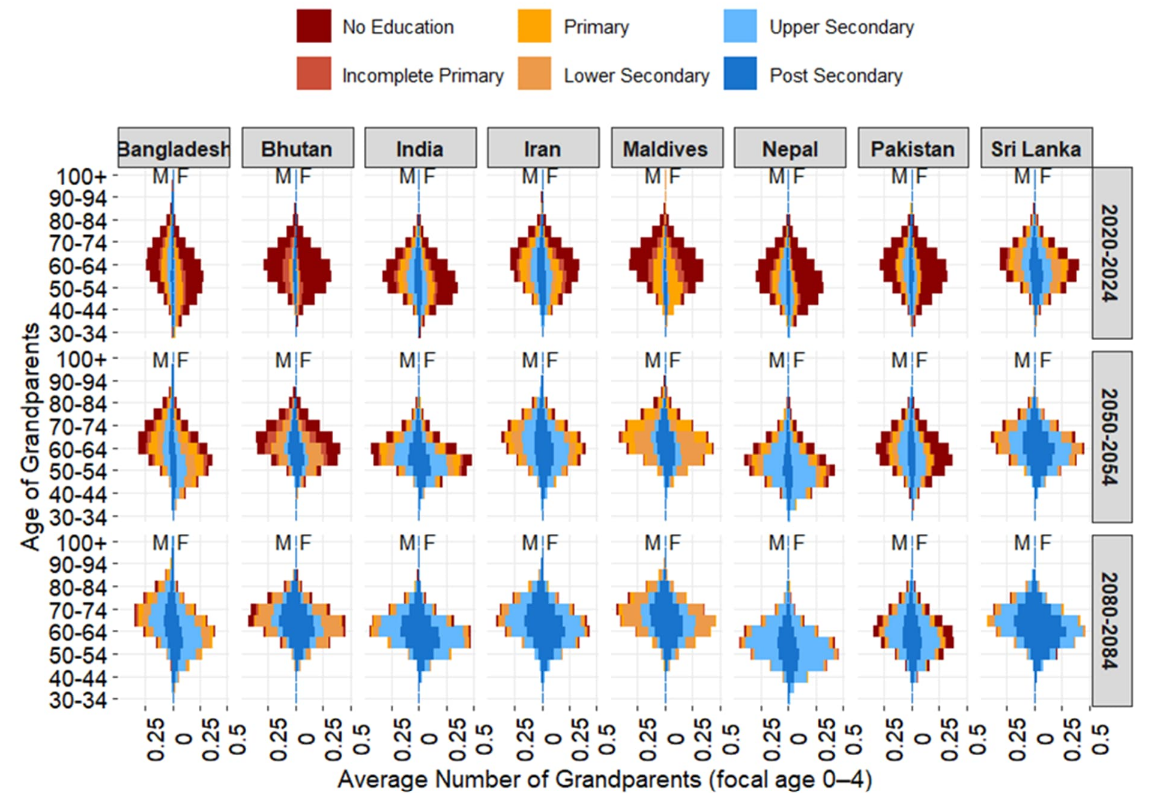
\includegraphics[width =1\textwidth]{figures/kin_ageedu_gm_bothsex_Nepal.pdf}
     \end{figure}    
\end{frame}

\begin{frame}{Kin loss by cause of death\fcite{schluter_youth_2024}}
          \begin{figure}[!h]
      \centering
      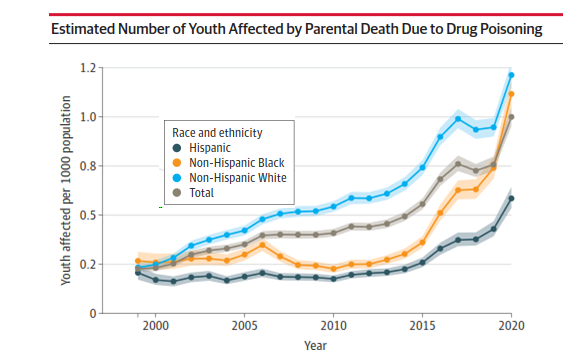
\includegraphics[width =.9\textwidth]{figures/arms.png}
     \end{figure}    
\end{frame}

\begin{frame}{Discuss}
    \begin{enumerate}
        \item Do you see any application of the kinship models to your own work? 
        \item Which model specification would be more appropriate for this?
    \end{enumerate}
\end{frame}

\end{document}




